\documentclass[hyperref=colorlinks]{beamer}
\mode<presentation>
\usetheme{iclpt}
\setbeamertemplate{navigation symbols}{}
\setbeamertemplate{headline}{
  \begin{beamercolorbox}[leftskip=.2cm,rightskip=.2cm,topskip=.2cm,ht=1.1cm,dp=0.1cm,wd=\textwidth]{institute in head/foot}
    
\includegraphics[height=1cm]{icl.pdf}
    \hfill
%    \includegraphics[height=1cm]{../Pics/ATLAS-Logo-Square-Blue-RGB.png}
%    
\includegraphics[height=1cm]{../Pics/CMS-Color.pdf}
    
\includegraphics[height=1cm]{TalkPics/t2k_logo_large.png}

%??put t2k logo here
  \end{beamercolorbox}
}
\setbeamertemplate{footline}{
  \begin{beamercolorbox}[ht=.35cm,dp=0.2cm,wd=\textwidth,leftskip=.3cm]{author in head/foot}%
    \begin{minipage}[c]{5cm}%
      \usebeamerfont{author in head/foot}
      \insertshortauthor 
      \insertshorttitle
    \end{minipage}\hfill%
    \hfill
    \insertframenumber{} / \ref{lastframe}
    %\hfill
    \begin{minipage}{6cm}
      \hfill
      %\insertshorttitle
    \end{minipage}
  \end{beamercolorbox}%
}

\definecolor{beamer@icdarkblue}{RGB}{0,51,102}
\definecolor{beamer@icmiddleblue}{RGB}{0,82,150} 
\definecolor{beamer@iclightblue}{RGB}{200,212,232}
\definecolor{beamer@icmiddlered}{RGB}{204,51,0}
\definecolor{beamer@iclightred}{RGB}{232,212,32}

\usepackage{tikz}
\usetikzlibrary{arrows,shapes,backgrounds}
\usepackage{color}
\usepackage{tabularx,colortbl}
\usepackage{graphicx}
\usepackage{pdfpages}
\usepackage{feynmp}
\usepackage{rotating}
\usepackage{moresize}
\usepackage{slashed}
\usepackage{xcolor,colortbl}
\DeclareGraphicsRule{*}{mps}{*}{}
\hypersetup{colorlinks=false}

\title[MaCh3 status]{\vspace{-0.2cm} MaCh3 Summer 17 OA}
\author[P. Dunne]{Patrick Dunne, \\ for the MaCh3 group}
\titlegraphic{
  \vspace{-0.4cm}
}
\date{}
\begin{document}
\tikzstyle{every picture}+=[remember picture]
\tikzstyle{na} = [baseline=-.5ex]
\begin{fmffile}{t2ktemplatefeyndiags}


  %TITLE PAGE
  %20 mins + 5 questions
  \section{Title}
  \begin{frame}
    \titlepage
    \centering
    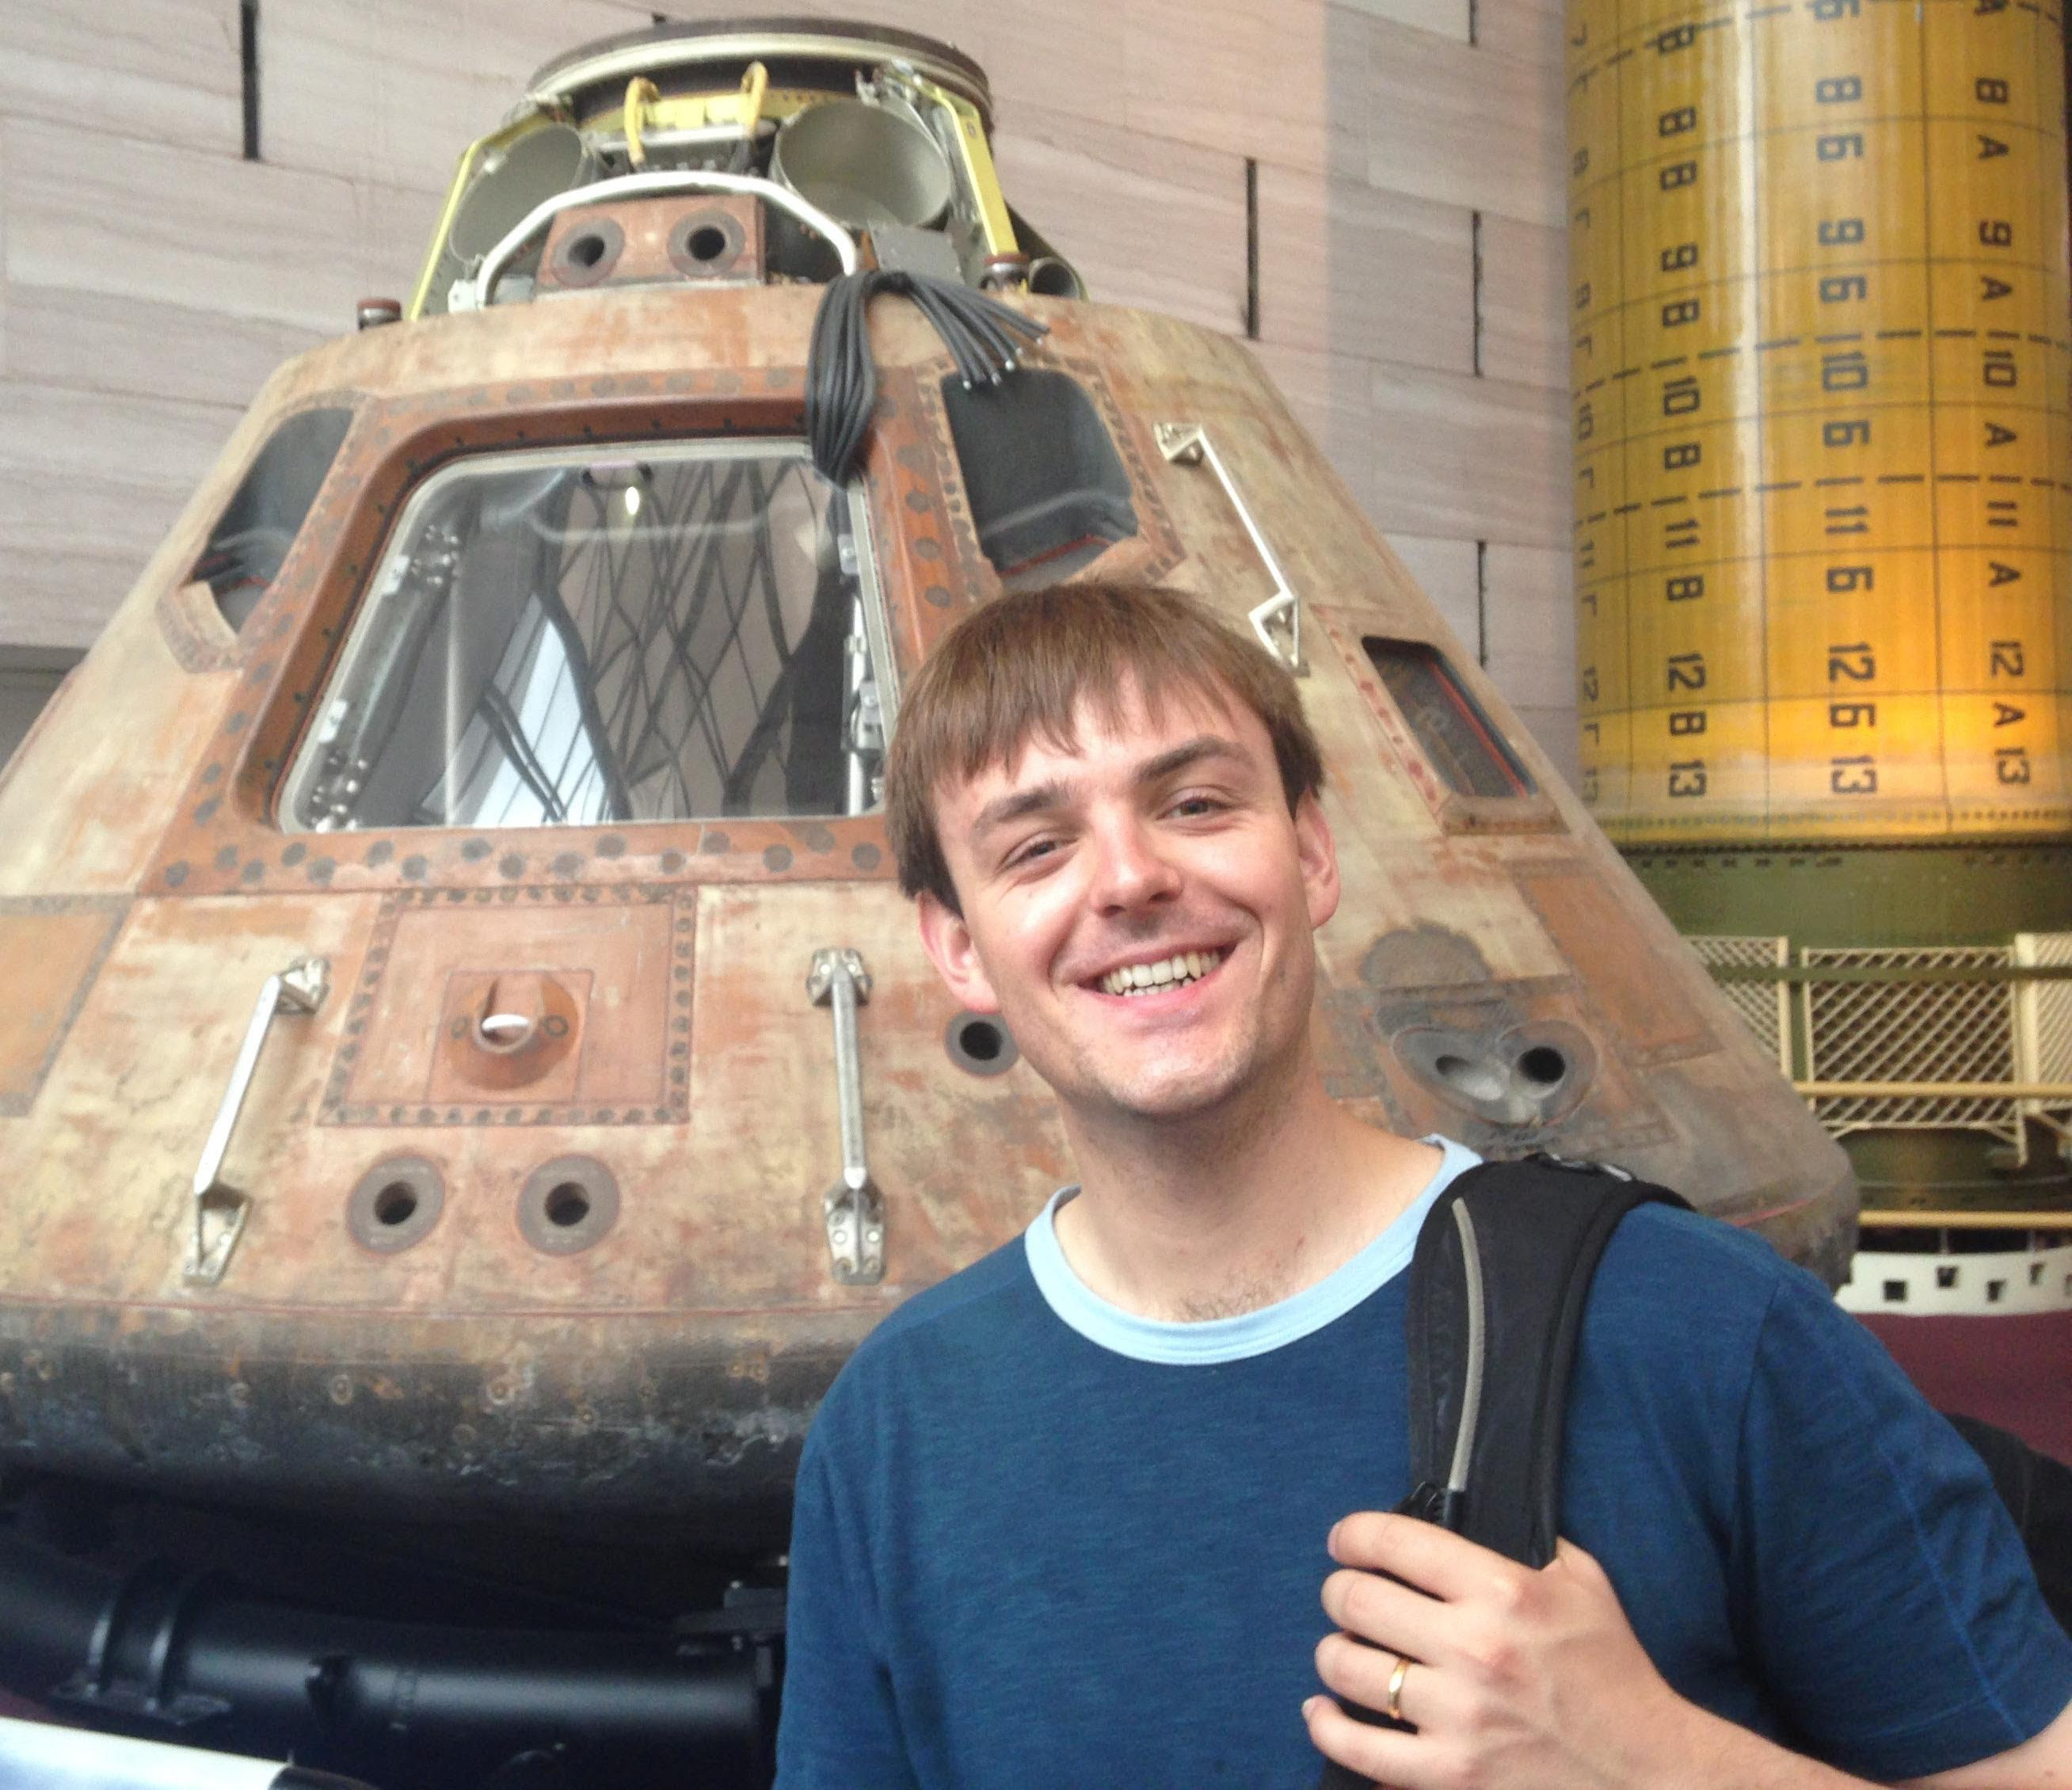
\includegraphics[width=.3\textwidth]{TalkPics/PdunneF2F050417/me.jpg}
  \end{frame}

  \begin{frame}
    \frametitle{Oscillations at T2K}
    \scriptsize
    \begin{itemize}
    \item Standard PMNS oscillations apply to mass eigenstates as:
    \end{itemize}
    \begin{equation*}
      \left(\begin{array}{c}
        \nu_{e}\\
        \nu_{\mu}\\
        \nu_{\tau}\\
  \end{array}\right)
      =
      \left(
      \begin{array}{ccc}
        1 & 0 & 0 \\
        0 & c_{23} & s_{23} \\
        0 & -s_{23} & c_{23} \\
      \end{array}
      \right)
      \left(
      \begin{array}{ccc}
        c_{13} & 0 & s_{13}e^{i\delta} \\
        0 & 1 & 0 \\
        -s_{13}e^{-i\delta} & 0 & c_{13} \\
      \end{array}
      \right)
      \left(
      \begin{array}{ccc}
        c_{12} & s_{12} & 0 \\
        -s_{12} & c_{12} & 0 \\
        0 & 0 & 1 \\
      \end{array}
      \right)      
      \left(
      \begin{array}{c}
        \nu_{1}\\
        \nu_{2}\\
        \nu_{3}\\
      \end{array}
      \right)
    \end{equation*}
    \begin{itemize}
    \item T2K sees disappearance of $\nu_{\mu}$, appearance of $\nu_{e}$ and equivalents for antineutrino
    \item Gives sensitivity to $\sin^2\left(\theta_{23}\right)$, $\sin^2\left(\theta_{13}\right)$, $\Delta m^2_{23}$ and $\delta$
    \end{itemize}
  \end{frame}

  \begin{frame}
    \frametitle{MaCh3 introduction}
    \begin{itemize}
    \item MaCh3 is a Bayesian Markov Chain Monte Carlo (MCMC) oscillation fitter
    \item Performs MCMC integration to give the posterior probability
    \item Choose to fit ND280 and SK simultaneously
    \end{itemize}
  \end{frame}



  \begin{frame}
    \frametitle{What goes into an oscillation fit?}
    \centering
    \includegraphics[width=.9\textwidth]{TalkPics/PdunneF2F050417/oadiagram.pdf}
    
    \scriptsize K. Duffy
  \end{frame}


  \begin{frame}
    \frametitle{Updates for Summer OA}
      \begin{itemize}
      \item SK data: Use full Run 1-8 SK data for all 5 samples
      \item[-] All analyses fitting in $E_{rec}$ for $\nu_{\mu}$ and 2D for $\nu_{e}$
      \item ND280 data: No new data, but new RHC binning
      \item New SK reconstruction using fitQun
      \item New xsec model
      \end{itemize}
      \centering
  \end{frame}

  \begin{frame}
    \frametitle{fitQun}
    \begin{itemize}
    \item SK reconstruction with significantly lower mis-ID probability
    \item Available for all samples used in OA fit
    \end{itemize}
    \centering
    \includegraphics[width=\textwidth]{TalkPics/PdunneF2F050417/fitqun.pdf}

    \scriptsize A. Missert
  \end{frame}

  \begin{frame}
    \frametitle{fitQun: Fiducial volume}
    \begin{columns}
      \column{.5\textwidth}
      \begin{itemize}
      \item Much lower mis-ID probability allows fiducial volume (FV) to be expanded
      \item Optimise 2 variables cut values based on:
        \begin{equation*}
          \sum^{bins}_{i} \frac{\left(\frac{dN_{i}}{d\theta}\right)}{N_{i}+\left(\sigma_{syst}^2\right)_{i}}
        \end{equation*}
      \item Results in 20\% larger FV with more events around oscillation max. energy
      \end{itemize}
      \column{.5\textwidth}
      \includegraphics[width=\textwidth]{TalkPics/PdunneF2F050417/fitqunfv.pdf}

      \scriptsize A. Missert
          
    \end{columns}
  \end{frame}


  \begin{frame}
    \frametitle{New xsec model (2017b)}
    \begin{itemize}
    \item Large changes made to this year's cross-section model:
    \item Removal of $E_{B}$ dial
    \item 2p2h uncertainty treatment
    \item Change to RPA treatment
    \end{itemize}
  \end{frame}
  
  \begin{frame}
    \frametitle{$E_{B}$}
    \begin{columns}
      \column{.5\textwidth}
      \begin{itemize}
      \item Part of model of inital nucleon momentum
      \item[-] Describes energy needed to remove nucleon from atom
      \item $E_{B}$ dial in 2015 parametrisation didn't migrate events as desired
      \item Also it's effect was very small, so we dropped it
      \end{itemize}
      \column{.5\textwidth}
      \includegraphics[width=\textwidth]{TalkPics/PdunneF2F050417/ebdiag.pdf}
    \end{columns}
  \end{frame}

  \begin{frame}
    \frametitle{$E_{B}$}
    \begin{columns}
      \column{.5\textwidth}
      \begin{itemize}
      \item Planned new dial based on comparison of nominal SF model with RFG model with varied $E_{B}$
      \item SF has larger phase space than RFG so should work
      \item Problem: larger $\neq$ covering
      \item[-] RFG (red) populates some areas SF (black) doesn't
      \item[-] Large bias in forward region
      \item Dropped new dial as well
      \end{itemize}
      \column{.5\textwidth}
      \includegraphics[width=\textwidth]{TalkPics/PdunneF2F050417/ebphasespace.pdf}
      
      \scriptsize M. Dunkman
    \end{columns}
  \end{frame}

  \begin{frame}
    \frametitle{2p2h}
    \begin{columns}
      \column{.5\textwidth}
      \begin{itemize}
      \item 2p2h is multi-nucleon hard scatter
      \item Effect largest at flux peak
      \item Old model only varied normalisation
      \item Add shape modelling
      \end{itemize}
      \column{.5\textwidth}
      \includegraphics[width=\textwidth]{TalkPics/PdunneF2F050417/2p2h.pdf}
    \end{columns}
  \end{frame}

  \begin{frame}
    \frametitle{BeRPA}
      \begin{itemize}
      \item RPA describes screening of nucleon by rest of nucleus
      \item Old model weighted to Nieves model nominal
      \item[-] No uncertainty
      \item Introduce BeRPA parametrisation
      \end{itemize}
      \begin{block}{}
        \vspace{-.4cm}
        \begin{equation*}
          \scriptsize
          f\left(x\right)=\begin{cases}
          A\left(1-\frac{x}{U}\right)^3+3B\left(1-\frac{x}{U}\right)^2\frac{x}{U}+3p_{1}\left(1-\frac{x}{U}\right)\left(\frac{x}{U}\right)^2+D\left(\frac{x}{U}\right)^3, x<U \\
          1+p_{2}\exp\left(-E\left(x-U\right)\right), x>U
          \end{cases}
        \end{equation*}
        \end{block}
        \normalsize
        \begin{itemize}
        \item Values and errors for A, B, D, E and U obtained by fitting to Nieves model
        \item[-] $p_{1}$ and $p_{2}$ fixed by continuity
        \end{itemize}
  \end{frame}

  \begin{frame}
    \frametitle{BeRPA}
    \begin{columns}
      \column{.5\textwidth}
      \begin{itemize}
      \item A, B, D, E and U varied in ND280 Data fit
      \item Appear to go away from nominal
      \item High flux parameters seen last year return to normal
      \item NB MaCh3 implement BeRPA event-by-event, other fitters don't
      \end{itemize}
      \column{.5\textwidth}
      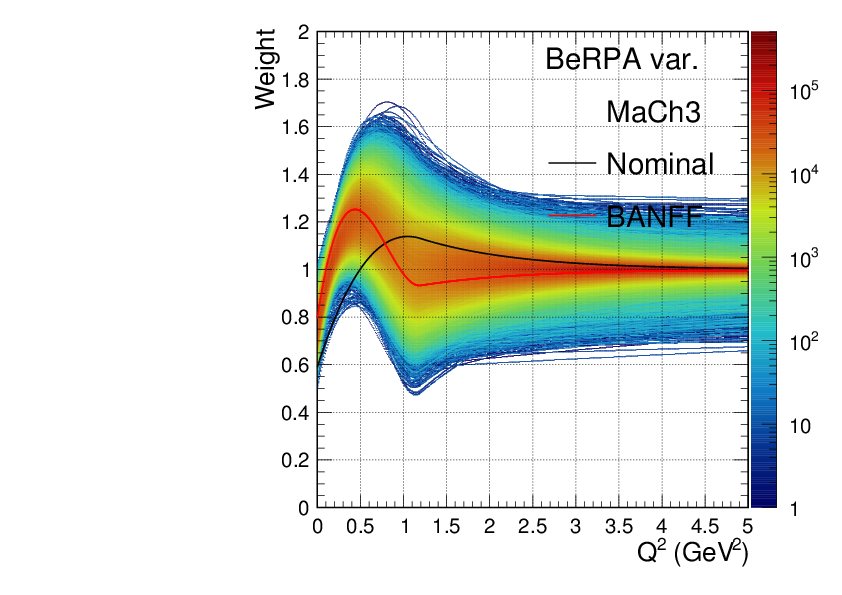
\includegraphics[clip=true,trim=250 0 0 0,width=\textwidth]{TalkPics/PdunneF2F050417/2017b_datafit_vanilla_BeRPA.png}

      \scriptsize C. Wret
    \end{columns}
  \end{frame}
  
  
  
  \begin{frame}
    \frametitle{Validation progress: event rate}
    \begin{itemize}
    \item All of the above changes implemented in MaCh3
    \item Validate that code is ok by checking against other analyses
    \item[-] expect some differences due to BeRPA treatment
    \item[-] Still validating CC1pi
    \end{itemize}
    \begin{columns}
      \column{.6\textwidth}
    \begin{block}{}
      \centering
      \begin{tabular}{|l|cc|}
        \hline
        & MaCh3 & p-theta \\
        \hline
        FHC 1Rmu & 145.817 & 148.031 \\
        FHC 1Re & 41.050 & 41.6955 \\
        RHC 1Rmu & 8.468 & 8.494 \\
        RHC 1Re & 67.039 & 68.0174 \\
        FHC CC1pi & 3.9659 & 3.63896\\
        \hline
      \end{tabular}
    \end{block}
    \end{columns}
  \end{frame}

  \begin{frame}
    \frametitle{Validation progress}
    \begin{itemize}
    \item Validate systematic model implementation too
    \item MaCh3 (dashed) vs p-theta (solid)
    \item[-] Expect small differences due to different spline binning
    \end{itemize}
    \includegraphics[width=.5\textwidth]{TalkPics/PdunneF2F050417/systvariation.pdf}
    \includegraphics[width=.5\textwidth]{TalkPics/PdunneF2F050417/systvariation2.pdf}

    
  \end{frame}

  \begin{frame}
    \frametitle{Asimov fits}
    \begin{itemize}
    \item Hot off the presses!
    \item woRC Asimov A ($\delta=-1.601$,  $\sin^2\left(\theta_{23}\right)=0.523$), Run 1-7 POT
    \end{itemize}
    %??Asimov plot
    \centering
    \vspace{-.2cm}
    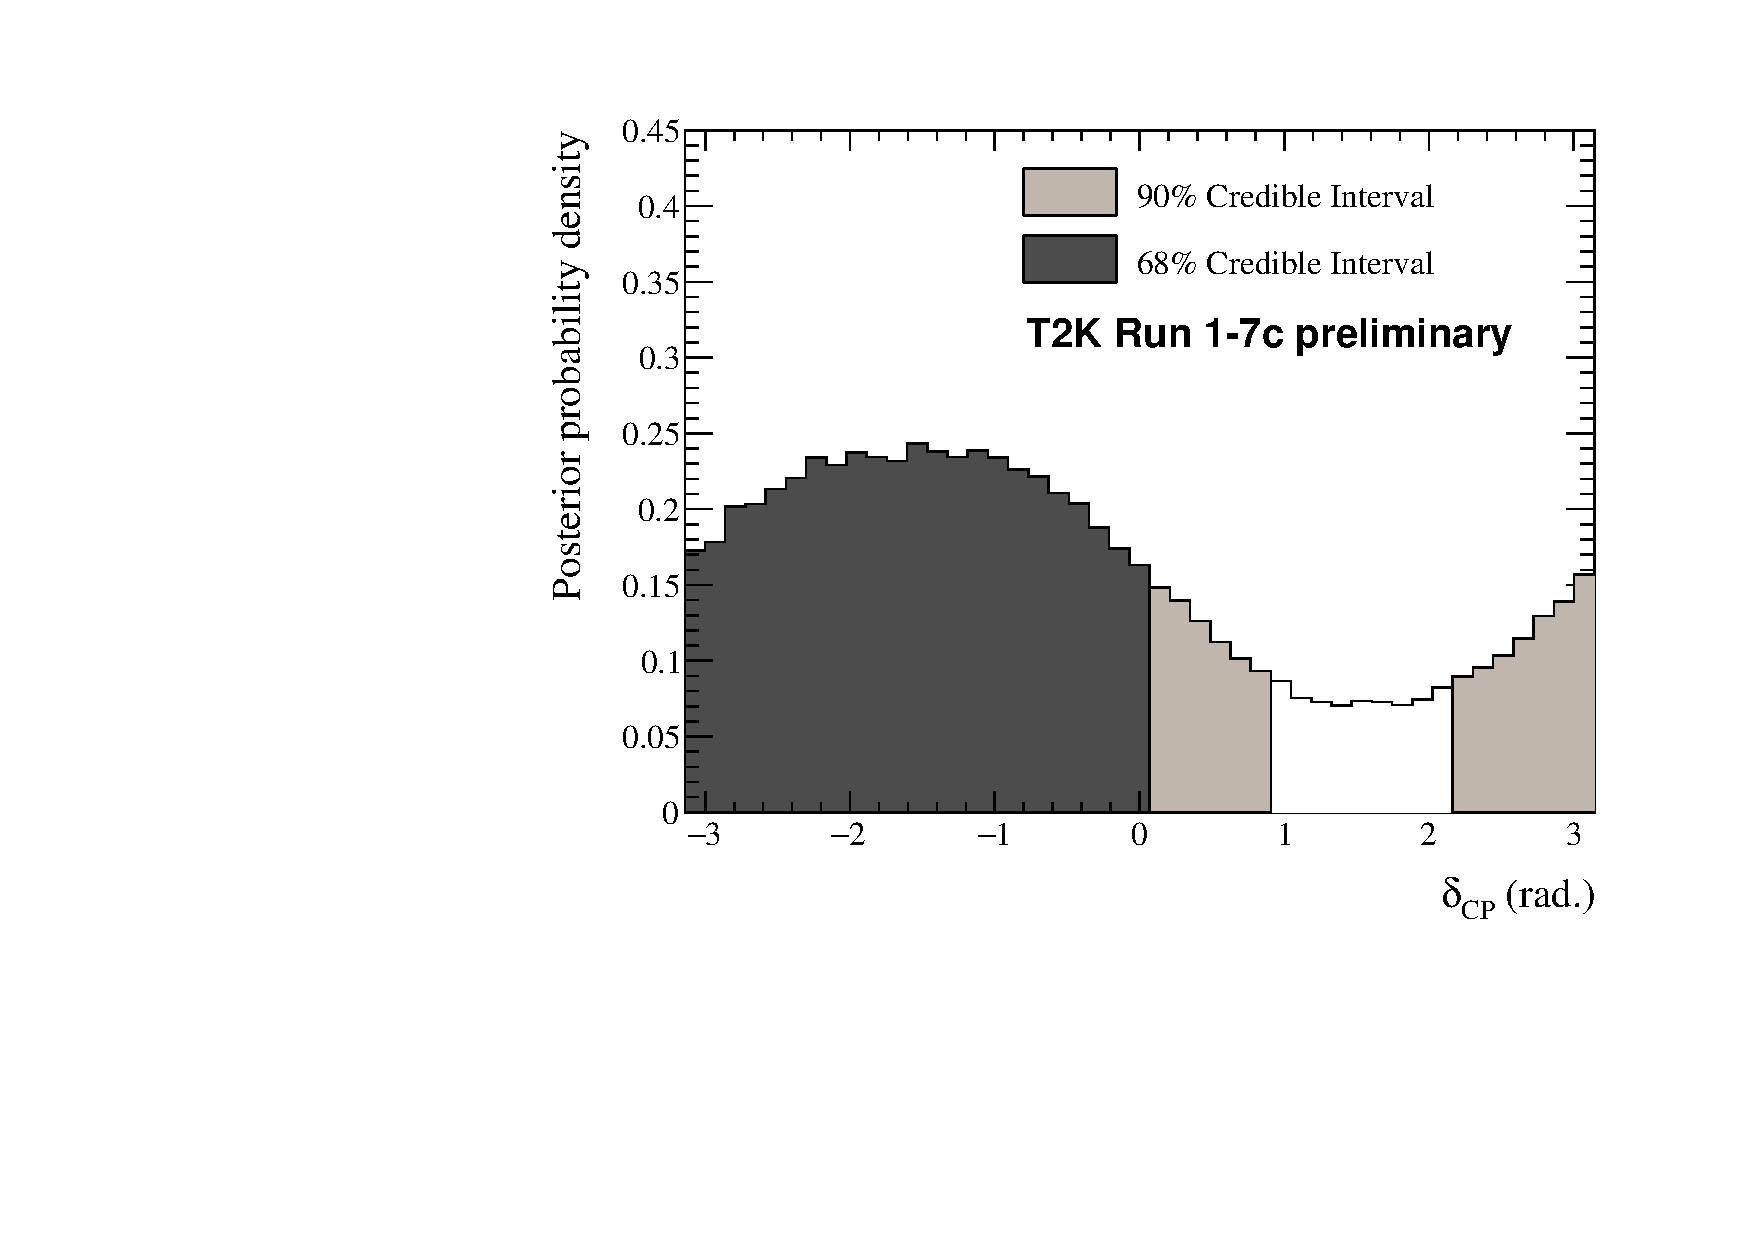
\includegraphics[width=.7\textwidth]{TalkPics/PdunneF2F050417/contours_woRC_asimovset12d/contours_1D_dcp_both_official.pdf}
  \end{frame}
  
  \begin{frame}
    \frametitle{Asimov fits: Comparison with p-theta}
    %??include comparison and comment
    \begin{itemize}
    \item Only 900k steps for MaCh3 (usually a few million)
    \item MaCh3 and p-theta using different ND fits which stills how some disagreement
    \end{itemize}
    \centering
    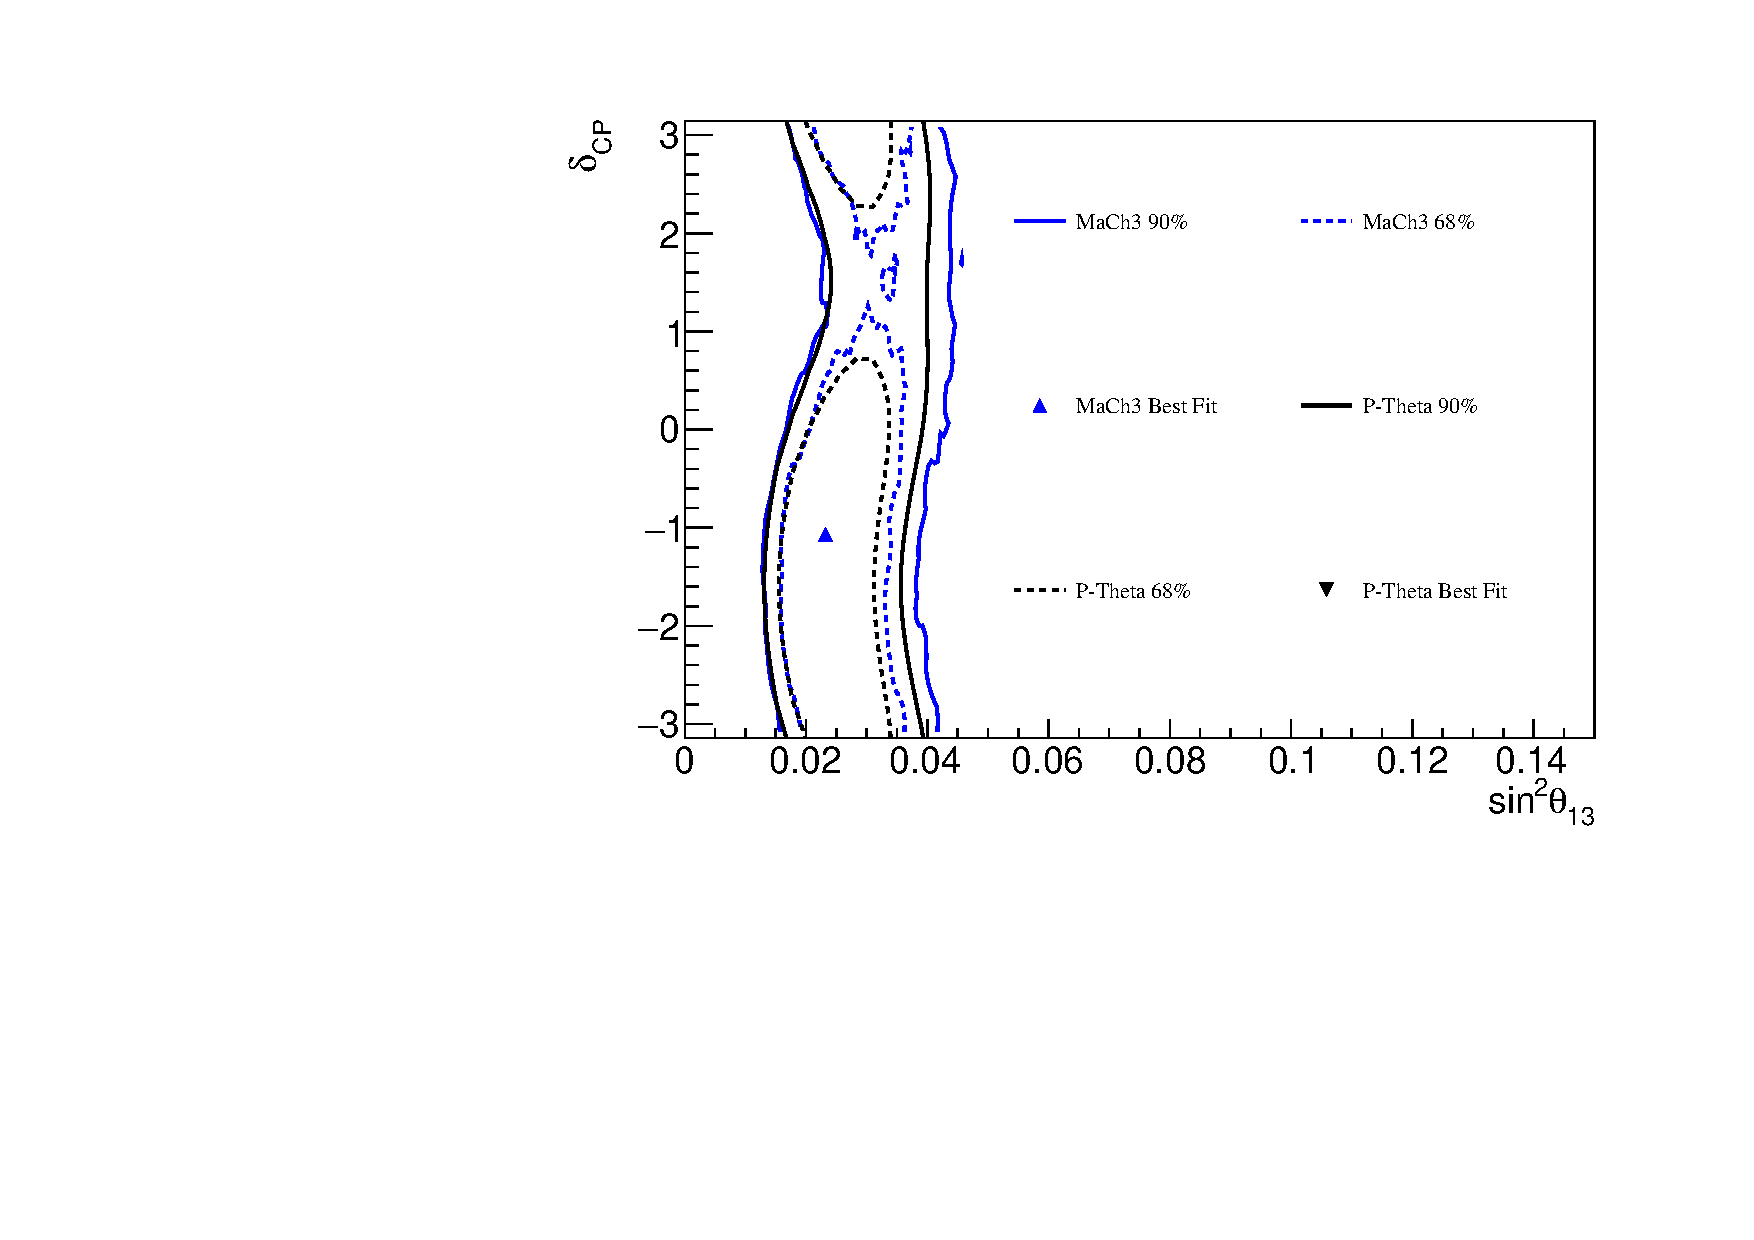
\includegraphics[width=.7\textwidth]{TalkPics/PdunneF2F050417/comparedcontours_datafit2D_mach3valor/comparedcontours_2D_mach3valor_woRC_th13dcp_NH.pdf}
  \end{frame}

  \begin{frame}
    \frametitle{Timeline}
    \begin{itemize}
    \item Targeting EPS-HEP: July 5-12
    \item Currently on time (just)
    \end{itemize}
    \centering
      \includegraphics[width=.5\textwidth]{TalkPics/OAupdate_160317/oaschedule.pdf}    
  \end{frame}
  
  \begin{frame}
    \frametitle{Conclusions}
    \label{lastframe}
    \begin{block}{}
      \begin{itemize}
      \item Lots of new features coming in summer OA
      \item[-] Improved xsec model
      \item[-] New SK reconstruction which allows expanded FV
      \item Still work to do and timeline is tight
      \item Excited to see the new data
        %??add some conclusions
       \end{itemize}
    \end{block}
  \end{frame}

  %Backup goes here
  

\begin{frame}
  \centering
  \huge \textcolor{beamer@icmiddleblue}{Backup}
\end{frame}

\end{fmffile}
\end{document}
